% XeLaTeX can use any Mac OS X font. See the setromanfont command below.
% Input to XeLaTeX is full Unicode, so Unicode characters can be typed directly into the source.

% The next lines tell TeXShop to typeset with xelatex, and to open and save the source with Unicode encoding.

%!TEX TS-program = xelatex
%!TEX encoding = UTF-8 Unicode

\documentclass[11pt]{article}
\usepackage{geometry}                % See geometry.pdf to learn the layout options. There are lots.
\geometry{margin=1.7cm,top=1.0cm,bottom=2.0cm}
\geometry{letterpaper}                   % ... or a4paper or a5paper or ... 
%\geometry{landscape}                % Activate for for rotated page geometry
\usepackage[parfill]{parskip}    % Activate to begin paragraphs with an empty line rather than an indent
\usepackage{graphicx}
\usepackage{amssymb}

\usepackage[compact]{titlesec}
\titlespacing{\section}{0pt}{2ex}{1ex}
\titlespacing{\subsection}{0pt}{1ex}{0ex}
\titlespacing{\subsubsection}{0pt}{0.5ex}{0ex}

% use case command
\usepackage{booktabs}

\newcommand\addrow[2]{#1 &#2\\ }

\newcommand\addheading[2]{#1 &#2\\ \hline}
\newcommand\tabularhead{\begin{tabular}{lp{0.8\linewidth}}
\hline
}

\newcommand\addmulrow[2]{\begin{minipage}[t][][t]{2.5cm}#1\end{minipage}% 
   &\begin{minipage}[t][][t]{0.8\linewidth}
    \begin{enumerate} #2   \end{enumerate}
    \end{minipage}\\ }

\newenvironment{usecase}{\tabularhead}
{\hline\end{tabular}}

% Will Robertson's fontspec.sty can be used to simplify font choices.
% To experiment, open /Applications/Font Book to examine the fonts provided on Mac OS X,
% and change "Hoefler Text" to any of these choices.

\usepackage{fontspec,xltxtra,xunicode}
\defaultfontfeatures{Mapping=tex-text}
\setromanfont[Mapping=tex-text]{Hoefler Text}
\setsansfont[Scale=MatchLowercase,Mapping=tex-text]{Gill Sans}
\setmonofont[Scale=MatchLowercase]{Andale Mono}

\title{Final Project Specification: Miller's Hollow Online}
\author{Team \textbf{Miller's Hollow}
\\Yiyun Yao(yiyuny) \& Jin Wang(jinw2) \& Shangjie Chen(shangjic)}
\date{}                                           % Activate to display a given date or no date

\begin{document}
\maketitle

\section{Functionality}
\subsection{Not in a Game}
\subsubsection{Authentication}
\begin{enumerate}
\item
Login: Registered Users may login to the website by correct username and password, and get authenticated and authorized
\item
Register: Unregistered Users may register to the website by providing username, password and email
\item
Activate Account: Registered User may activate the account by click the activation link in the email automatically sent when successfully registered
\item
Logout: Authenticated User may logout the website
\item
Change Password: Authenticated User may change the password by correct current password
\item
Reset Password: User who forget their password may reset the password by providing the email correspond to the account
\item
Reset Password Confirm: User may set their new password by click the link in the email automatically sent when password is successfully reset
\end{enumerate}

\subsubsection{Profiling \& Setting}
\begin{enumerate}
\item
Editing User Information: Authenticated User may change the first name, last name and email
\item
Upload avatar: Authenticated User may upload a picture to change the avatar
\item
Set preference game: Authenticated User may set the preference game in the settings to skip the game choose phase in build game and matching game
\item
Set waiting time: Authenticated User may set the waiting time in the settings to change the default waiting time before every speech starts
\item
Set Music, Display and Log settings: Authenticated User may set the music volume, display settings(turn on/off camera of other user in case the network is not good enought) and log verbosity in the settings
\end{enumerate}

\subsubsection{Game Mode}
\begin{enumerate}
\item
Matching Game: Authenticated User may start a matching game where different unrelated players attend
\item
Build Room Game: Authenticated User may build a room game where friends are invited to play game together; in the mean time, a share token is generated for other users to join
\item
Join Room Game: Authenticated User may join a room game by a share token
\end{enumerate}

\begin{figure}
\centering
\begin{minipage}{.5\linewidth}
\centering
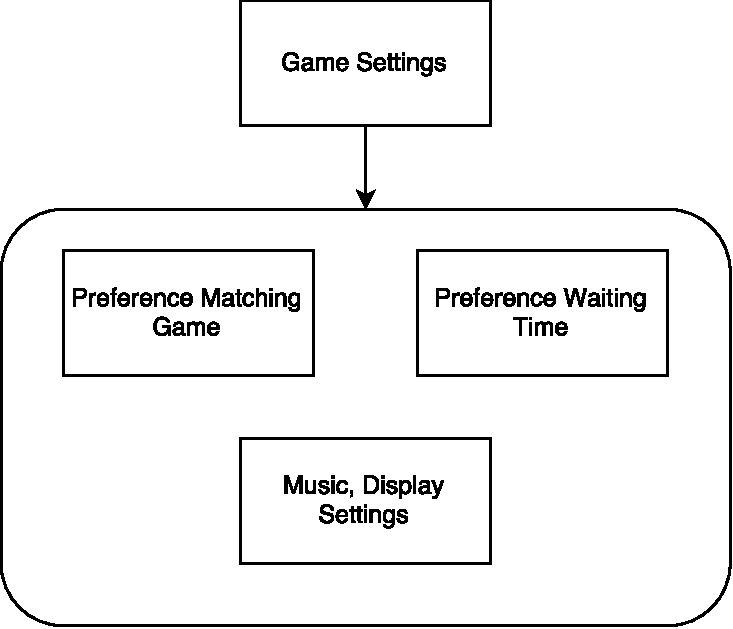
\includegraphics[width=.9\linewidth]{func-settings.pdf}
\caption{Functionality: Profiling \& Setting}
\label{fig:func-settings}
\end{minipage}%
\begin{minipage}{.5\linewidth}
\centering
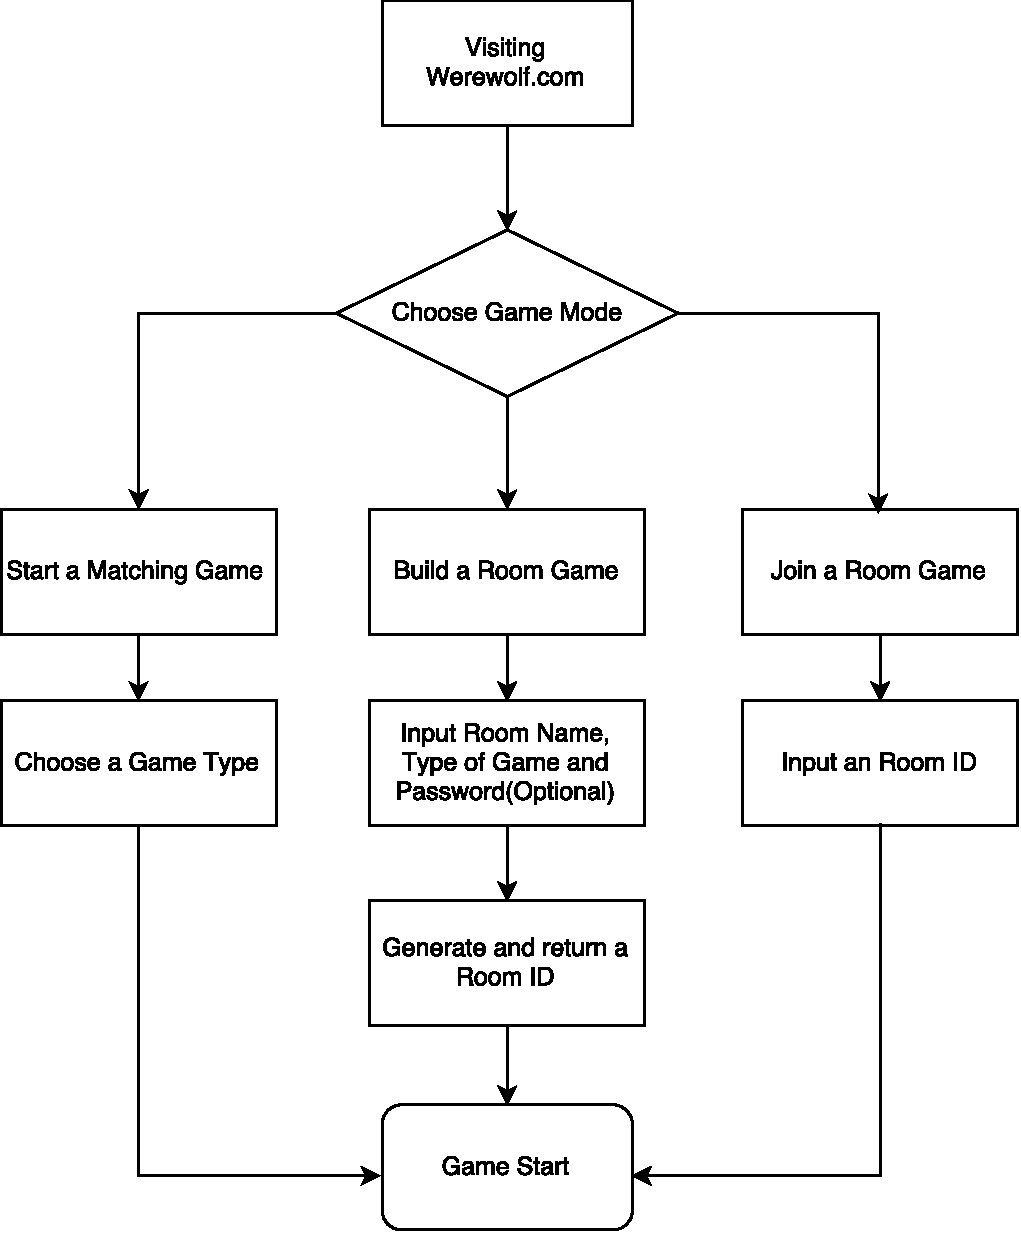
\includegraphics[width=.9\linewidth]{func-index.pdf}
\caption{Functionality: Game Mode}
\label{fig:func-index}
\end{minipage}
\end{figure}

\subsubsection{Room Member}
When Authenticated User join a Room Game, he/she automatically becomes a Room Member
\begin{enumerate}
\item
Change to empty seat: Room Member may change the seat to a new one if it is empty
\item
Leave the room: Room Member may leave the room by clicking the Leave Button
\item
Chat: Room Member may chat in the room and the message can be seen by all the Room Members
\item
Get ready: Room Member may get ready by clicking the Ready Button(when all the Room Member is ready, the Room Owner can Start the game)
\item
Cancel ready: Room Member who is ready may cancel it by clicking the Cancel Button
\end{enumerate}

\subsubsection{Room Owner}
Room Owner have the functionality of Room Member from 1 to 3. A Room Member can be selected as a Room Owner by the previous Room Owner. The original one is the user who build the room. A Room Game can only have one Room Owner. Room Owner has the extra functionalities as follow.
\begin{enumerate}
\item
Set a Room Member as Room Owner: Room Owner may choose another user as the new Room Owner
\item
Kickout Room Member: Room Owner may kickout Room member
\item
Start Game: Room Owner may start the Room Game by clicking Start Button when all the Room Member is ready
\end{enumerate}

\subsubsection{Achievements \& Tasks}
\begin{enumerate}
\item
Tasks: Authenticated User may receive one task a day automatically in the Achievements \& Tasks Board, and get awards by completing it. One user can hold three tasks at max
\item
Exchange task: Authenticated User may exchange a task one day, the new one will be different from the old one
\item
Winning Rate: Authenticated User may check the winning rate in the Achievements \& Tasks Board
\item
Time Played: Authenticated User may check the time played in the Achievements \& Tasks Board
\item
Level: Authenticated User may check the level in the Achievements \& Tasks Board, which is mainly based on the winning rate and time played. The level is the main dependency of Matching Game.
\end{enumerate}

\begin{figure}
\centering
\begin{minipage}{.6\linewidth}
\centering
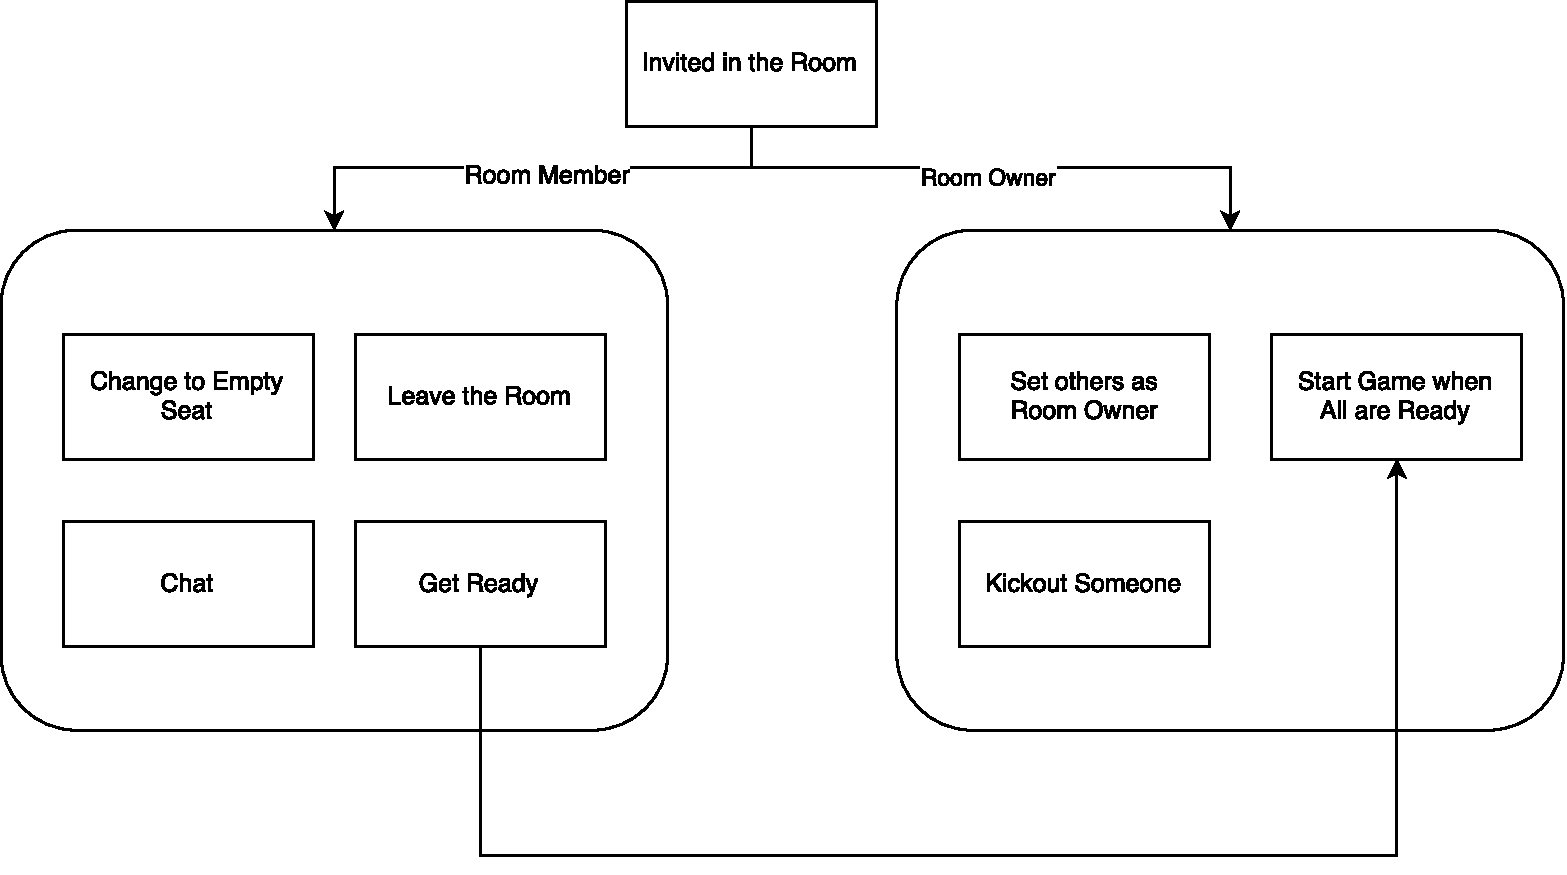
\includegraphics[width=.9\linewidth]{func-inroom.pdf}
\caption{Functionality: Room Member \& Room Owner}
\label{fig:func-inroom}
\end{minipage}%
\begin{minipage}{.4\linewidth}
\centering
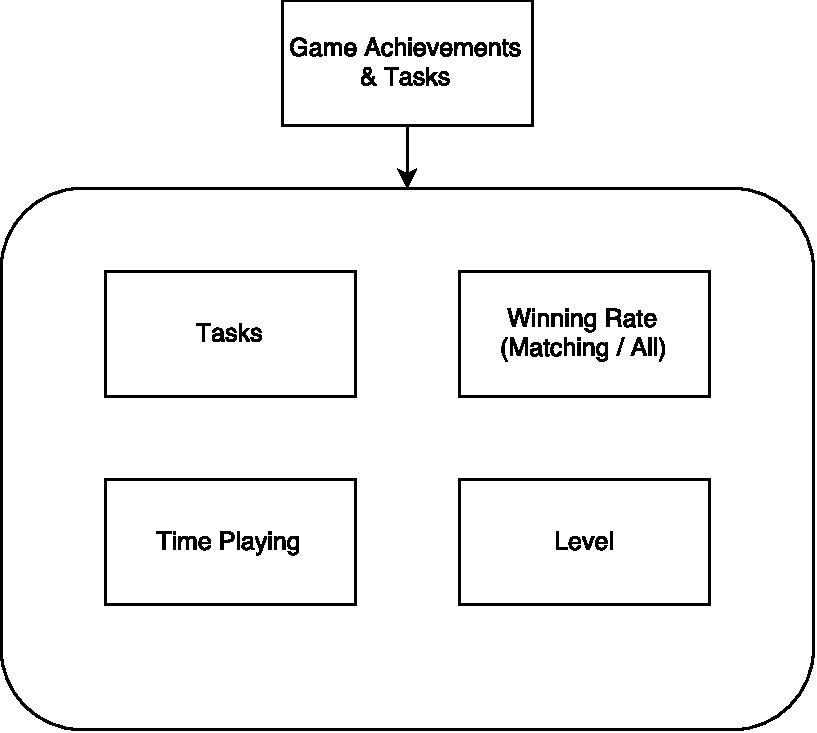
\includegraphics[width=.9\linewidth]{func-tasks.pdf}
\caption{Functionality: Achievements \& Tasks}
\label{fig:func-tasks}
\end{minipage}
\end{figure}

\subsection{In a Game}

\begin{figure}
\centering
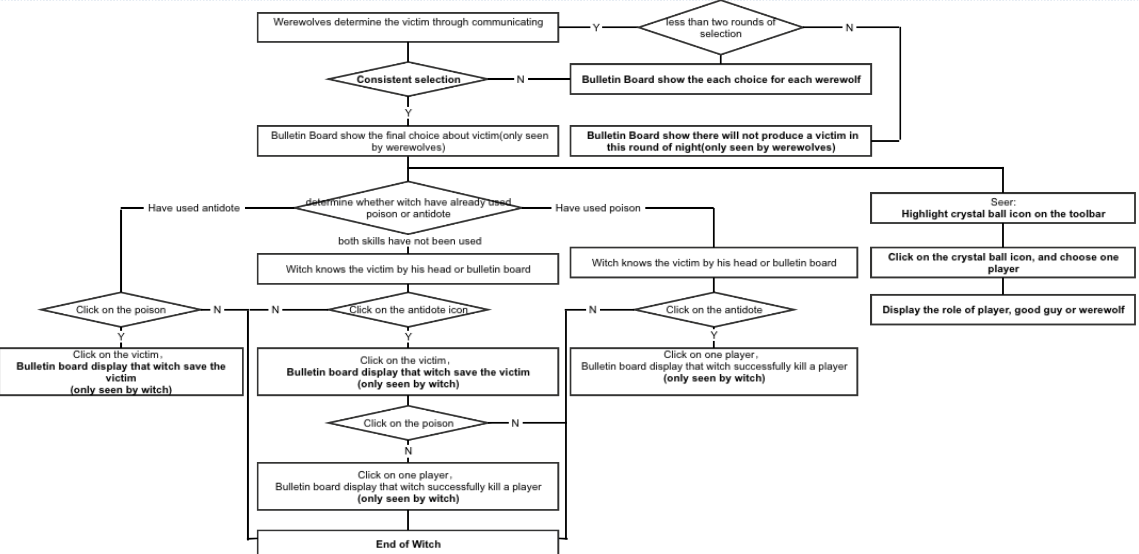
\includegraphics[width=0.9\linewidth, keepaspectratio]{func-gamenight.png}
\caption{Functionality: Game in the Night}
\label{fig:func-gamenight}
\end{figure}

\section{Data Model}


% For many users, the previous commands will be enough.
% If you want to directly input Unicode, add an Input Menu or Keyboard to the menu bar 
% using the International Panel in System Preferences.
% Unicode must be typeset using a font containing the appropriate characters.
% Remove the comment signs below for examples.

% \newfontfamily{\A}{Geeza Pro}
% \newfontfamily{\H}[Scale=0.9]{Lucida Grande}
% \newfontfamily{\J}[Scale=0.85]{Osaka}

% Here are some multilingual Unicode fonts: this is Arabic text: {\A السلام عليكم}, this is Hebrew: {\H שלום}, 
% and here's some Japanese: {\J 今日は}.



\end{document}  